\question Two very long, thin wires run perpendicular to one another and eventually cross as shown in the figure below. The wires do not come into conductive contact when they cross. In this problem, use the standard coordinate system where $\hat{x}$ points to the right ($\rightarrow$), $\hat{y}$ points upward ($\uparrow$), and $\hat{z}$ points out of the page ($\bigodot$).

A known current $I_1=3\ \mathrm{A}$ flows upward (in the $+\hat{y}$ direction) in the vertically oriented wire. The current in the horizontal wire is unknown (you know neither direction or magnitude).

You measure the magnetic field at two different points: point $A$ is a distance $d=3\ \mathrm{cm}$ to the right of the vertically oriented wire and a distance $d$ above the horizontal wire. Point $B$ is a distance $d$ to the \textit{left} of the vertical wire, and a distance $d$ above the horizontal wire.


\begin{center}
	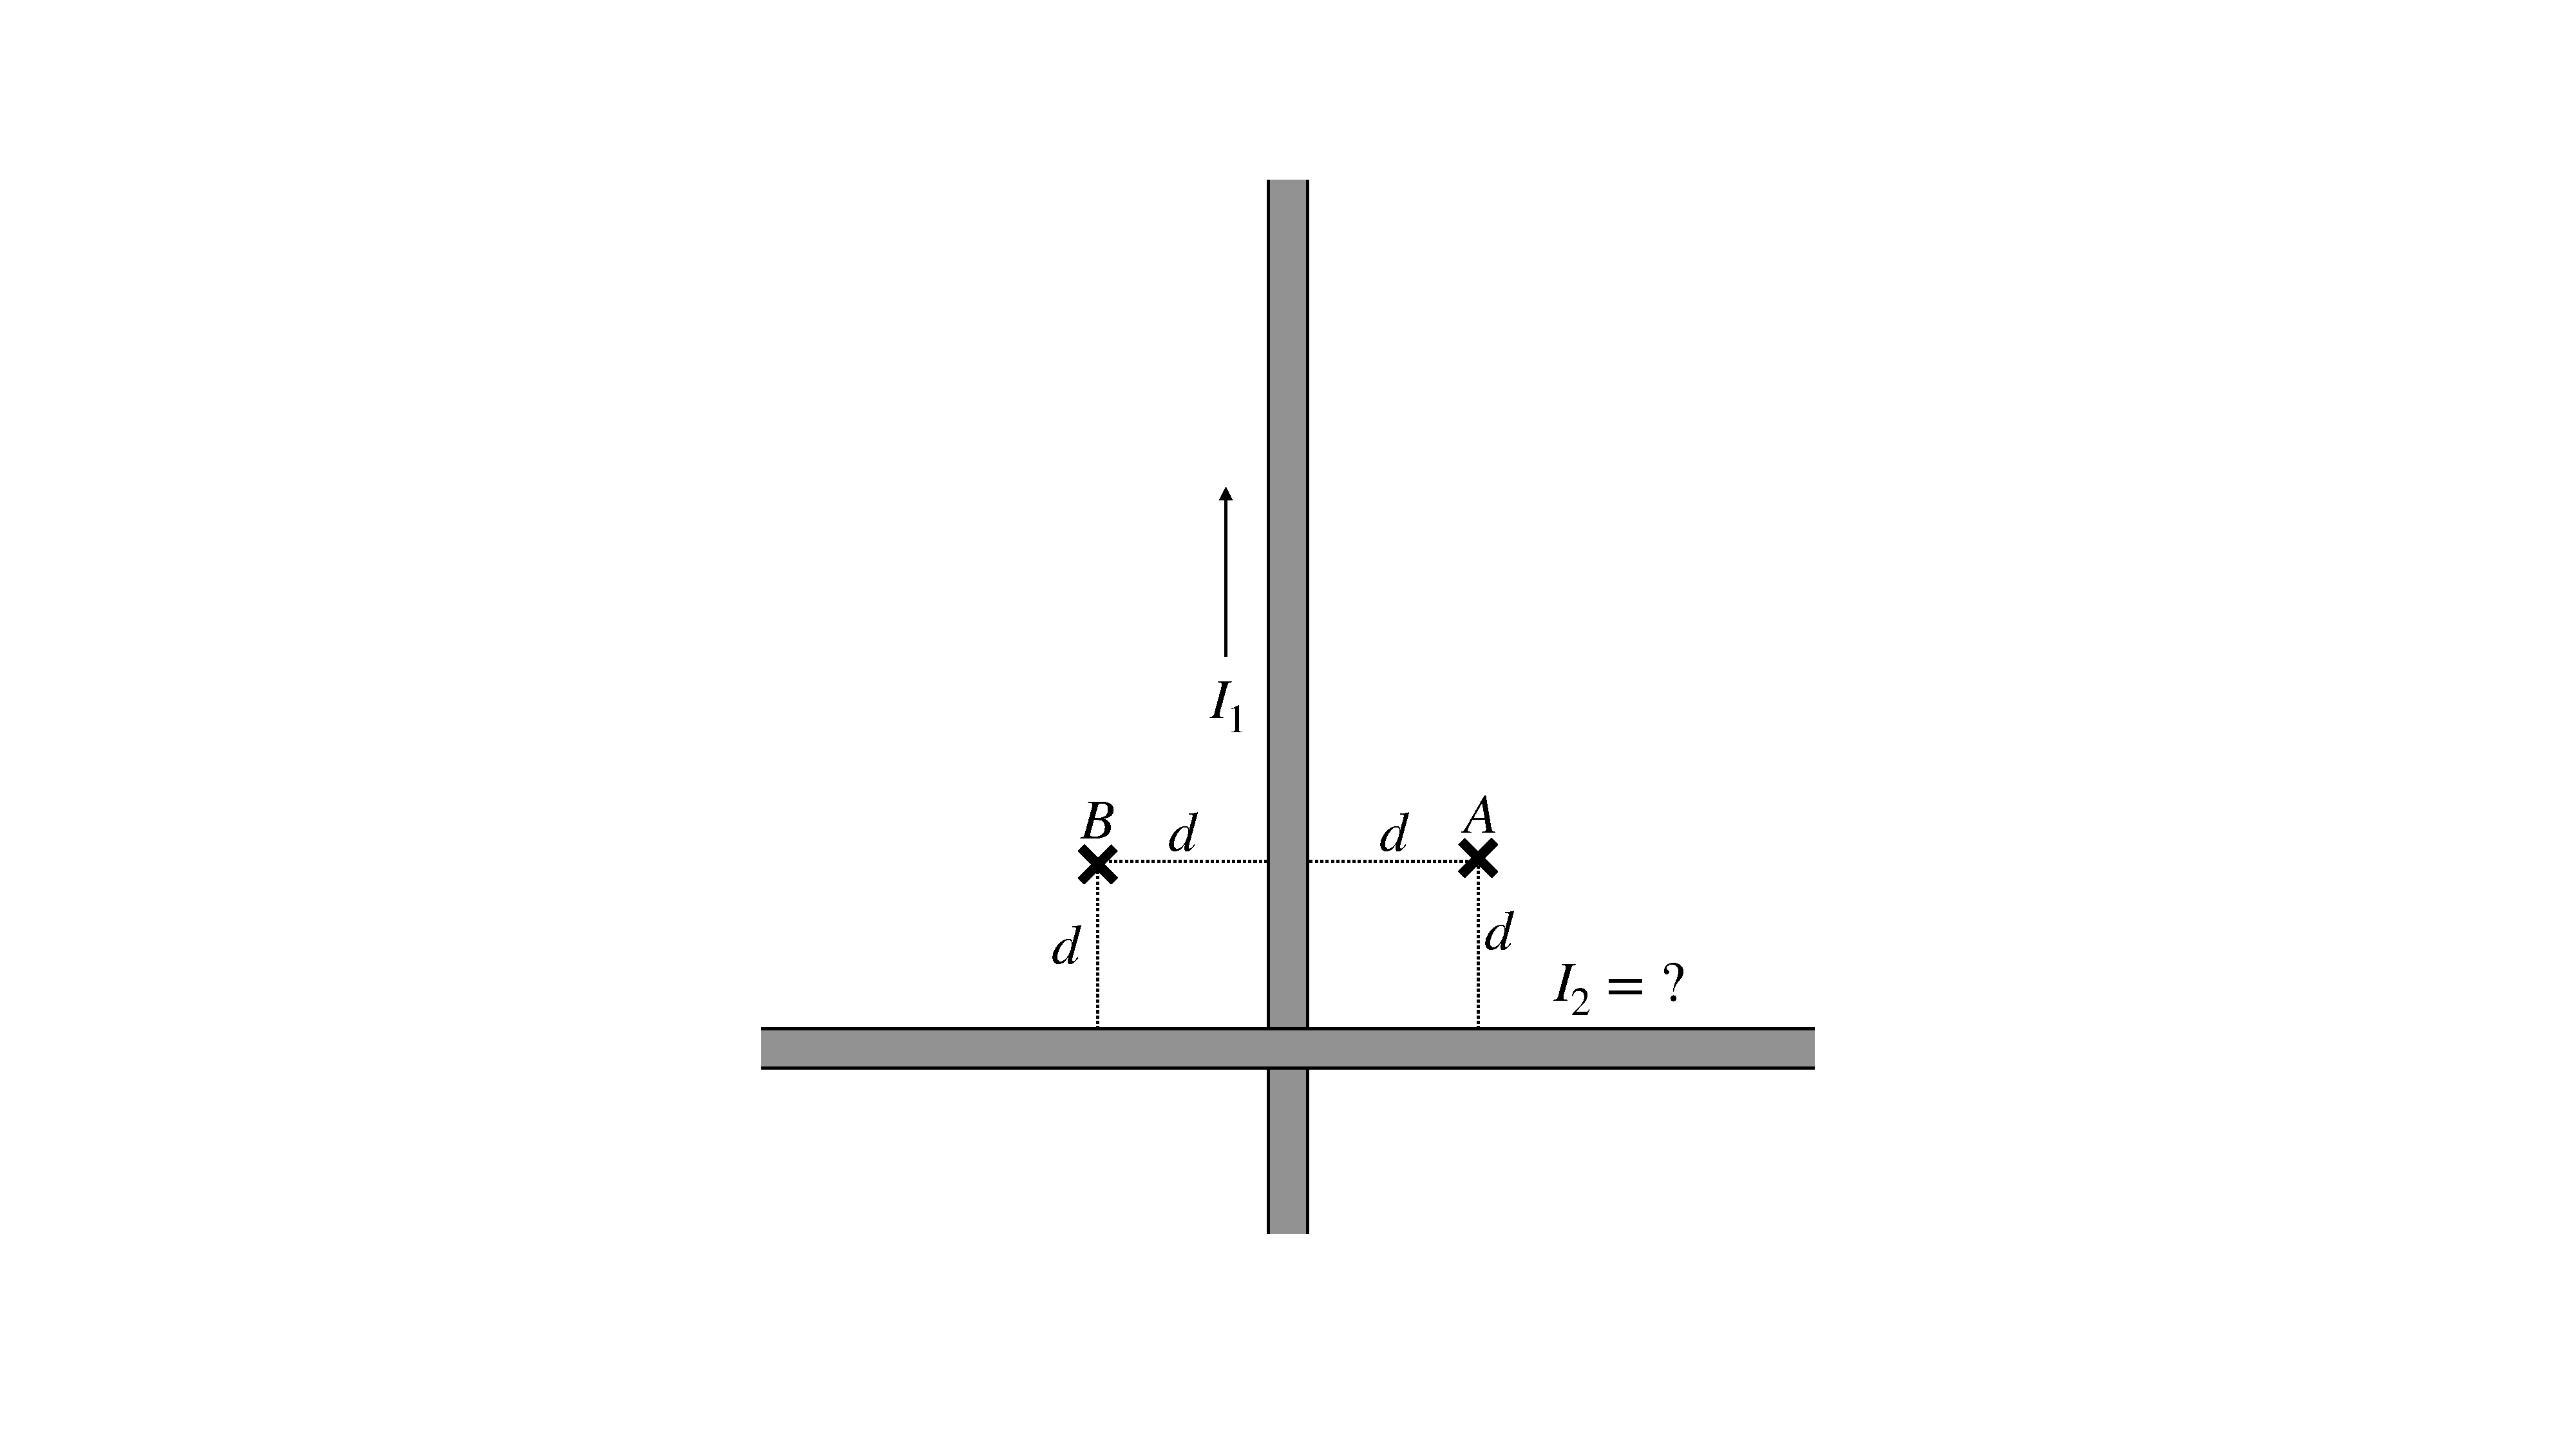
\includegraphics[width=.4\textwidth]{perp_wires.pdf}
\end{center}


You measure the magnetic field at point $A$ and find that it is zero at that location.
\begin{parts}
	\part[10] Based on this information, what is the current $I_2$? Specify both the value and the direction.
	\vspace{5cm}
	\part[10] What is the magnetic field at point $B$?
\end{parts}